\documentclass[12pt, twoside]{article}
\usepackage[letterpaper, margin=1in, headsep=0.5in]{geometry}
\usepackage[english]{babel}
\usepackage[utf8]{inputenc}
\usepackage{amsmath}
\usepackage{amsfonts}
\usepackage{amssymb}
\usepackage{tikz}
%\usetikzlibrary{quotes, angles}

\usepackage{graphicx}
\usepackage{enumitem}
\usepackage{multicol}

\usepackage{fancyhdr}
\pagestyle{fancy}
\fancyhf{}
\renewcommand{\headrulewidth}{0pt} % disable the underline of the header

\fancyhead[RE]{\thepage}
\fancyhead[RO]{\thepage \\ Name: \hspace{3cm}}
\fancyhead[L]{BECA / Dr. Huson / 10th Grade Geometry\\* Unit 7: Analytic Geometry Review\\15 February 2019}

\begin{document}
\subsubsection*{Pop Quiz: Operations on the coordinate plane}
  \begin{enumerate}

  \item The line $l$ has the equation $y=-\frac{1}{2} x+3$.
    \begin{enumerate}
      \item What is the slope of the line $k$, given $k \parallel l$?
      \vspace{1.3cm}
      \item What is the slope of the line $m$, given $m \perp l$?
      \vspace{1.3cm}
    \end{enumerate}

  In the following two problems, solve for the value of $x$.
    \begin{multicols}{2}
      \item   $\frac{1}{3}(6x-9)=17$ \vspace{4cm}
      \item   $\frac{1}{4}(5-x)=2$ \vspace{4cm}
    \end{multicols}
      \vspace{4cm}

  \item Given $f(x)=3x+3$. Simplify $f(2)$. \vspace{2.5cm}
  \item Given $g(x)=\frac{1}{2} x-1$. Solve for $x$ such that for $g(x)=2$. \vspace{4cm}


  \item Write down the center and radius of each circle.
    \begin{enumerate}
      \begin{multicols}{2}
      \item   $(x-1)^2+(y-7)^2=64$
      \item   $(x+3)^2+(y-2)^2=9^2$
      \end{multicols}
    \end{enumerate}

\newpage

  \item Convert this quadratic function from vertex form to standard form ($f(x)=x^2+bx+c$) by expanding the squared term and simplifying.

      \[f(x) = (x+5)^2-15\]
  \vspace{3cm}

  \item Graph and label the two equations. Mark their intersection as an ordered pair.
    \begin{multicols}{2}
      $y = \frac{3}{4}x-2$ \\
      $2x+3y = 12$
    \end{multicols}     \vspace{2cm}
    Are the lines parallel, perpendicular, or neither? Justify your answer.
    \vspace{2cm}

    \begin{center} %4 quadrant regents grid w T-Chart
    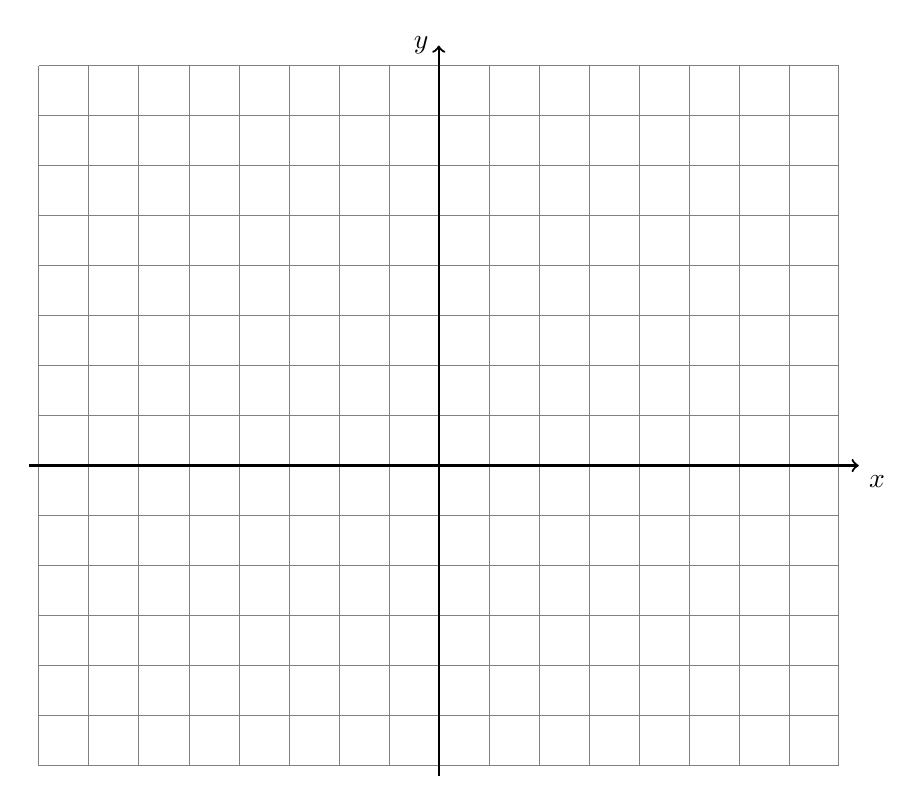
\begin{tikzpicture}[scale=.635]
      \draw [help lines] (-8,-6) grid (8,8);
      \draw [thick, ->] (-8.2,0) -- (8.4,0) node [below right] {$x$};
      \draw [thick, ->] (0,-6.2)--(0,8.4) node [left] {$y$};
    \end{tikzpicture}
    \end{center}

  \end{enumerate}
\end{document}
